%%%%%%%%%%%%%%%%%%%%%%%%%%%%%%%%%%%%%%%%%
% Wenneker Assignment
% LaTeX Template
% Version 2.0 (12/1/2019)
%
% This template originates from:
% http://www.LaTeXTemplates.com
%
% Authors:
% Vel (vel@LaTeXTemplates.com)
% Frits Wenneker
%
% License:
% CC BY-NC-SA 3.0 (http://creativecommons.org/licenses/by-nc-sa/3.0/)
% 
%%%%%%%%%%%%%%%%%%%%%%%%%%%%%%%%%%%%%%%%%

%----------------------------------------------------------------------------------------
%	PACKAGES AND OTHER DOCUMENT CONFIGURATIONS
%----------------------------------------------------------------------------------------

\documentclass[11pt, parskip=half]{scrartcl} % Font size

%%%%%%%%%%%%%%%%%%%%%%%%%%%%%%%%%%%%%%%%%
% Wenneker Assignment
% Structure Specification File
% Version 2.0 (12/1/2019)
%
% This template originates from:
% http://www.LaTeXTemplates.com
%
% Authors:
% Vel (vel@LaTeXTemplates.com)
% Frits Wenneker
%
% License:
% CC BY-NC-SA 3.0 (http://creativecommons.org/licenses/by-nc-sa/3.0/)
% 
%%%%%%%%%%%%%%%%%%%%%%%%%%%%%%%%%%%%%%%%%

%----------------------------------------------------------------------------------------
%	PACKAGES AND OTHER DOCUMENT CONFIGURATIONS
%----------------------------------------------------------------------------------------

\usepackage{amsmath, amsfonts, amsthm} % Math packages

\usepackage{geometry}

\usepackage{listings} % Code listings, with syntax highlighting

\usepackage[french]{babel} % English language hyphenation

\usepackage{graphicx} % Required for inserting images
\graphicspath{{Figures/}{./}} % Specifies where to look for included images (trailing slash required)

\usepackage{booktabs} % Required for better horizontal rules in tables

\usepackage{subcaption} % Required for creating figures with multiple parts (subfigures)

\usepackage{todonotes} % Required for inserting todo notes

\usepackage{array} % Required for customising tables

\usepackage{hyperref} % Required for adding links	and customising them

\numberwithin{equation}{section} % Number equations within sections (i.e. 1.1, 1.2, 2.1, 2.2 instead of 1, 2, 3, 4)
\numberwithin{figure}{section} % Number figures within sections (i.e. 1.1, 1.2, 2.1, 2.2 instead of 1, 2, 3, 4)
\numberwithin{table}{section} % Number tables within sections (i.e. 1.1, 1.2, 2.1, 2.2 instead of 1, 2, 3, 4)

\setlength\parindent{0pt} % Removes all indentation from paragraphs

\usepackage{enumitem} % Required for list customisation
\setlist{noitemsep} % No spacing between list items

%----------------------------------------------------------------------------------------
%	DOCUMENT MARGINS
%----------------------------------------------------------------------------------------

\usepackage{geometry} % Required for adjusting page dimensions and margins

\geometry{
	paper=a4paper, % Paper size, change to letterpaper for US letter size
	top=2.5cm, % Top margin
	bottom=3cm, % Bottom margin
	left=3cm, % Left margin
	right=3cm, % Right margin
	headheight=0.75cm, % Header height
	footskip=1.5cm, % Space from the bottom margin to the baseline of the footer
	headsep=0.75cm, % Space from the top margin to the baseline of the header
	%showframe, % Uncomment to show how the type block is set on the page
}

%----------------------------------------------------------------------------------------
%	FONTS
%----------------------------------------------------------------------------------------

\usepackage[utf8]{inputenc} % Required for inputting international characters
\usepackage[T1]{fontenc} % Use 8-bit encoding

\usepackage{fourier} % Use the Adobe Utopia font for the document

%----------------------------------------------------------------------------------------
%	SECTION TITLES
%----------------------------------------------------------------------------------------

\usepackage{sectsty} % Allows customising section commands

\sectionfont{\vspace{6pt}\centering\normalfont\scshape} % \section{} styling
\subsectionfont{\normalfont\bfseries} % \subsection{} styling
\subsubsectionfont{\normalfont\itshape} % \subsubsection{} styling
\paragraphfont{\normalfont\scshape} % \paragraph{} styling

%----------------------------------------------------------------------------------------
%	HEADERS AND FOOTERS
%----------------------------------------------------------------------------------------

\usepackage{scrlayer-scrpage} % Required for customising headers and footers

\ohead*{} % Right header
\ihead*{} % Left header
\chead*{} % Centre header

\ofoot*{} % Right footer
\ifoot*{} % Left footer
\cfoot*{\pagemark} % Centre footer
 % Include the file specifying the document structure and custom commands
\geometry{a4paper, margin=0.8in}

%----------------------------------------------------------------------------------------
%	TITLE SECTION
%----------------------------------------------------------------------------------------

\title{	
	\normalfont\normalsize
	\large\textsc{Sorbonne Université, UFR de Physique}\\ % Your university, school and/or department name(s)
	\vspace{2pt} % Whitespace
	\normalsize Master 1 : Physique fondamentale et applications\\
	\vspace{25pt} % Whitespace
	\rule{\linewidth}{0.5pt}\\ % Thin top horizontal rule
	\vspace{20pt} % Whitespace
	{\huge Projet IA : Le Modèle d'Ising}\\ % The assignment title
	\vspace{2pt} % Whitespace
	{Intelligence artificielle pour la physique}\\
	\vspace{12pt} % Whitespace
	\rule{\linewidth}{2pt}\\ % Thick bottom horizontal rule
	\vspace{12pt} % Whitespace
}

\author{\LARGE A. Cremel-Schlemer \large (3800159) \\ \LARGE G. Carvalho \large (xxxxxxxx) \\ \LARGE M. Panet \large (28705836)} % Your name

\date{\normalsize\today} % Today's date (\today) or a custom date

\begin{document}

\maketitle % Print the title
\tableofcontents % Print the contents

\newpage

\addcontentsline{toc}{section}{Introduction}
\section*{Introduction}

Le modèle d'Ising est un modèle de physique statistique introduit par Rudolph Peierls, Wilhelm Lenz et Ernst Ising dans les années 1920. Ce modèle d'une remarquable simplicité lui permet pourtant de mettre en exergue un comportement de transition de phase. \par


Sous sa formulation historique, le modèle d'Ising permet d'étudier la transition de phase paramagnétique/ferromagnétique d'un matériau. 
Certains matériaux possèdent une aimantation intrinsèque ; ils sont dits ferromagnétiques. C'est le cas des aimants. Cette propriété provient d'interactions à courte portée entre les spins d'un cristal. Mais, comme l'a découvert en 1895 le physicien Pierre Curie, ces matériaux perdent leur propriété magnétique au-dessus d'une température caractéristique appelée température de Curie $T_C$.
On trouve aussi des matériaux dits paramagnétiques. Ces matériaux ne sont pas magnétiques, mais le deviennent au contact d'un champ magnétique extérieur puissant.
En l'absence de champ magnétique extérieur, les spins de ces matériaux sont désordonnés, de sorte qu'en moyenne, le moment magnétique du matériau est nul : le materiaux n'est pas magnétique. Sous l'action d'un champ magnétique extérieur, ces moments se polarisent, ce qui rend le matériau magnétique.

L'hamiltonien du modèle d'Ising prend donc en compte ces deux propriétés, puisqu'une partie de cet est relative à l'interaction ferromagnétique à courte portée et l'autre partie est relative à l'interaction de chaque spin du cristal avec un champ magnétique extérieur. 
Dans la plupart des modèles numériques, on travaille sans champ extérieur.


La relative généralité de ce modèle (interactions locales et interaction individuelle avec une force extérieure) transcende la physique et permet de décrire qualitativement et parfois quantitativement une très grande variété de situations (paramagnétisme, gaz réticulaire, agents économiques, modèles écologiques, utilisation en analyse et traitement de l'image). Il donnera même lieu à un modèle plus général : le modèle de Potts (qui généralise l'aspect binaire du modèle d'Ising lié à la binarité des spins).


À travers notre exposé sur l'intelligence artificielle, nous allons nous intéresser à un jeu de données constitué de $16 000$ images issues d'une simulation numérique du modèle d'Ising 2D. Chaque image est associée à une température caractéristique allant de $0.25$ à $4$ (sans unité) et à un label. Le label renseigne sur la phase dans laquelle l'image se trouve. La \textit{phase ferromagnétique} est une phase où les spins sont globalement tous alignés ou forment des îlots de spins alignés ($|M| > 0$). Le label \textit{phase paramagnétique} rends compte du régime où les spins sont globalement désordonnés ($M = 0$).


Nous allons explorer différentes méthodes pour voir quelles solutions d'intelligence artificielle nous permettent de trancher, à partir d'une image donnée, si l'on est dans la phase paramagnétique ou ferromagnétique. Nous nous intéresserons aussi à la manière dont sont générées les données du modèle d'Ising. Nous chercherons à voir s'il est possible de prédire la température d'une image de manière fiable et même s'il est possible de générer de nouvelles données sans faire appel à une simulation numérique coûteuse.

\section{Génération de données}
Afin de mieux cerner le problème initiale, nous avons recréé la simulation du modèle d'Ising 2D pour des images $40 \times 40$ comme celle présente dans le dataset.
Le modèle d'Ising 2D est une approche numérique du problème posé en introduction où l'on fait l'hypothèse d'un cristal plat et de maille carrée pour lequel chaque atome est associé à un pixel d'une image.


Chaque spin est représenté soit par un 0, soit par un 1. Le 1 pour un spin Up, le 0 pour un spin Down. Pour améliorer la validité du modèle, des conditions aux bords périodiques sont utilisées. Concrètement cela revient à traiter la surface d'un tore qu'on aurait dépliée (cf. Figure \ref{fig:ising2D}). 

\begin{figure}[h]
	\begin{subfigure}{0.5\textwidth}
		\centering
		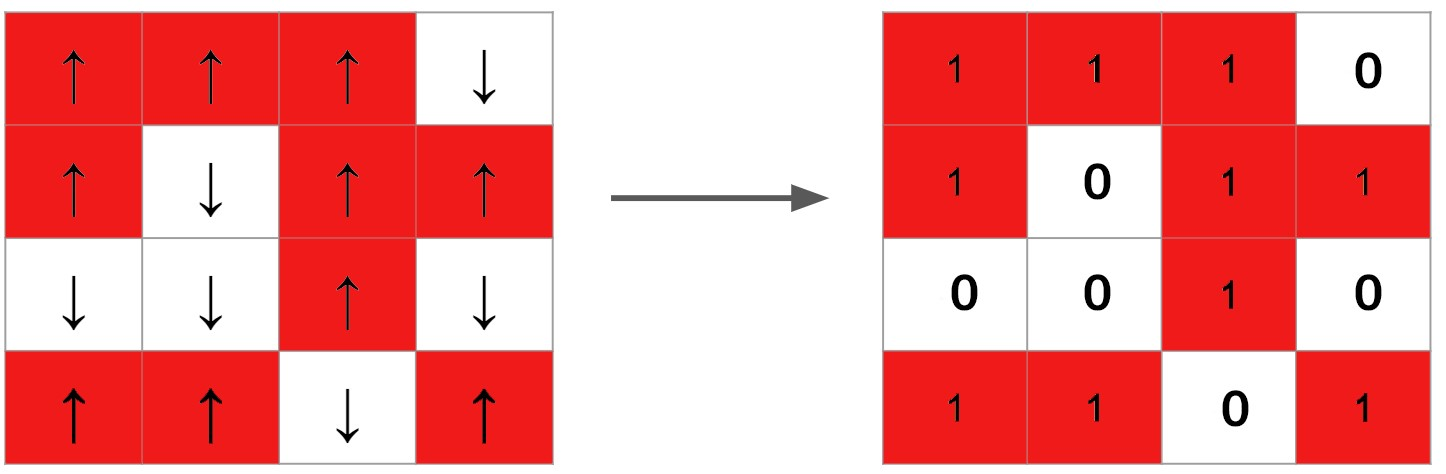
\includegraphics[width=0.95\linewidth]{./figures/torus_left.jpg}
		\caption{Les spins sont soit Up = 1, soit Down = 0}
	\end{subfigure}
	\begin{subfigure}{0.5\textwidth}
		\centering
		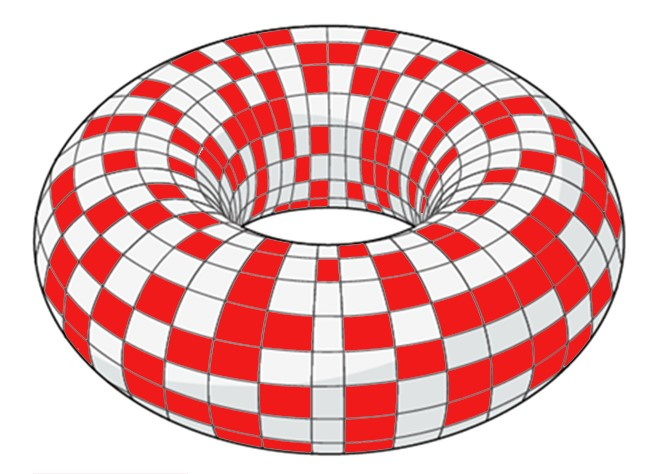
\includegraphics[width=0.5\linewidth]{./figures/torus_right.jpg}
		\caption{Conditions aux bords périodiques}
	\end{subfigure}
	\caption{Représentation du modèle d'Ising 2D}
	\label{fig:ising2D}
\end{figure}


Le Hamiltonien du problème est donnée par l'équation :

\begin{equation*}
    H = -J  \displaystyle \sum_{i,j}\sigma_{i}\sigma_{j} - h\displaystyle \sum_{i} \sigma_{i}
\end{equation*}

où $\sigma_{i} = \pm 1$. Celà dit, comme nous travaillons avec des $0$ et des $1$, il y a quelques manipulations à réaliser sur l'Hamiltonien. On fait de plus abstraction de la deuxième partie de l'hamiltonien qui traite du paramgnétisme.

Il nous reste donc qu'à traiter : 
\begin{equation*}
    H = -J  \displaystyle \sum_{i,j}(2\sigma_{i}-1)(2\sigma_{j}-1)
\end{equation*}

Que signifie cet Hamiltonien ? C'est un Hamiltonien de couplage entre spin. À priori, pour respecter la physique du système qu'on cherche à étudier, ce couplage ne se réalise qu'à courte portée, et donc que entre spin "plus proche voisin" puisqu'il s'agit d'une intéraction d'échange à courte portée. Par ailleurs, on choisie de travailler avec des constantes dimentionnées de sorte que: $\frac{J}{K_B}=1$

On va maintenant se rapprocher d'un des spins de notre modèle. Situé au centre, ses plus proches voisins forment une croix suisse autour de lui. On calcule son Hamiltonien local : 

\begin{equation*}
H_{local} = E_{ij} =  (2\sigma_{i}-1) \displaystyle \sum_{j}(2\sigma_{j}-1) = (2\sigma_{i}-1) \times \bigg[ 2\times( R + L + U + D ) -4 \bigg]
\end{equation*}
avec :

\begin{figure}[h]
	\centering
	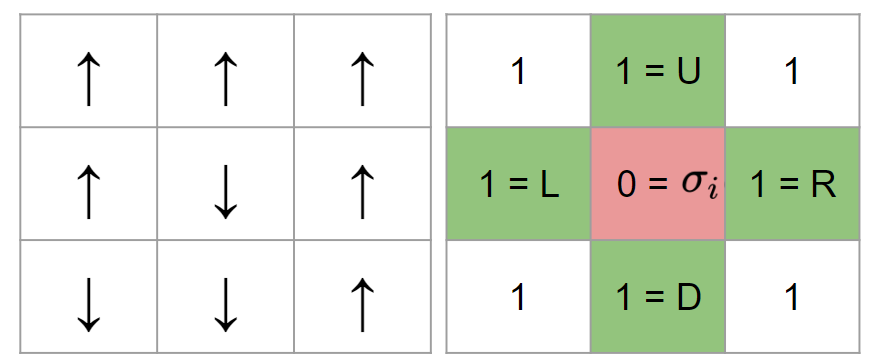
\includegraphics[width=0.5\linewidth]{H.png}
	\caption{Hamiltonien local}
	\label{fig:H}
\end{figure}

Partons d'un système idéal où tous les spins sont alignées. En raison de l'agitation thermique un spin aléatoire du cristal inverse son sens. La variation d'énergie associé à ce changement est donnée par : 
\begin{equation*}
\Delta E = E_f - E_i
\end{equation*}
Et la probabilité qu'un tel changement s'opère est proportionelle au poids de Boltzmann :  

\begin{equation*}
P(\Delta E) \propto e^{-\beta \Delta E} = e^{-\beta \Delta E}
\end{equation*}

L'idée est la suivante :  l'ordinateur va piocher une case au hasard calculer le $\Delta E$ associé. Ce $\Delta E$ ne peux prendre que 5 valeurs possibles : 
\begin{center}
\begin{tabular}{|l|m{4cm}|}
\hline
n voisin de sens opposé & $\Delta E $\\
\hline
0 & 8\\
1 & 4\\ 
2 & 0\\ 
3 & -4\\
4 & -8\\\hline

\end{tabular}
\end{center}

\vspace{4mm}

 Dans le cas ou $\Delta E \in \{0,-4,-8\}$ l'energie est minimisée donc le changement s'opère naturellement, l'ordinateur change le pixel d'état.
 Dans le cas inverse, c'est à dire  $\Delta E \in \{4,8\}$ un nombre aléatoire $x$ tiré selon une distribution uniforme entre 0 et 1 et est comparer à $e^{-\beta \Delta E}$.
 Si $x < e^{-\beta \Delta E}$ alors l'ordinateur change le pixel d'état. Sinon il ne le fait pas.

 On remarque que plus T est important plus la probabilité de transition est importante.

\begin{figure}[h]
	\centering
	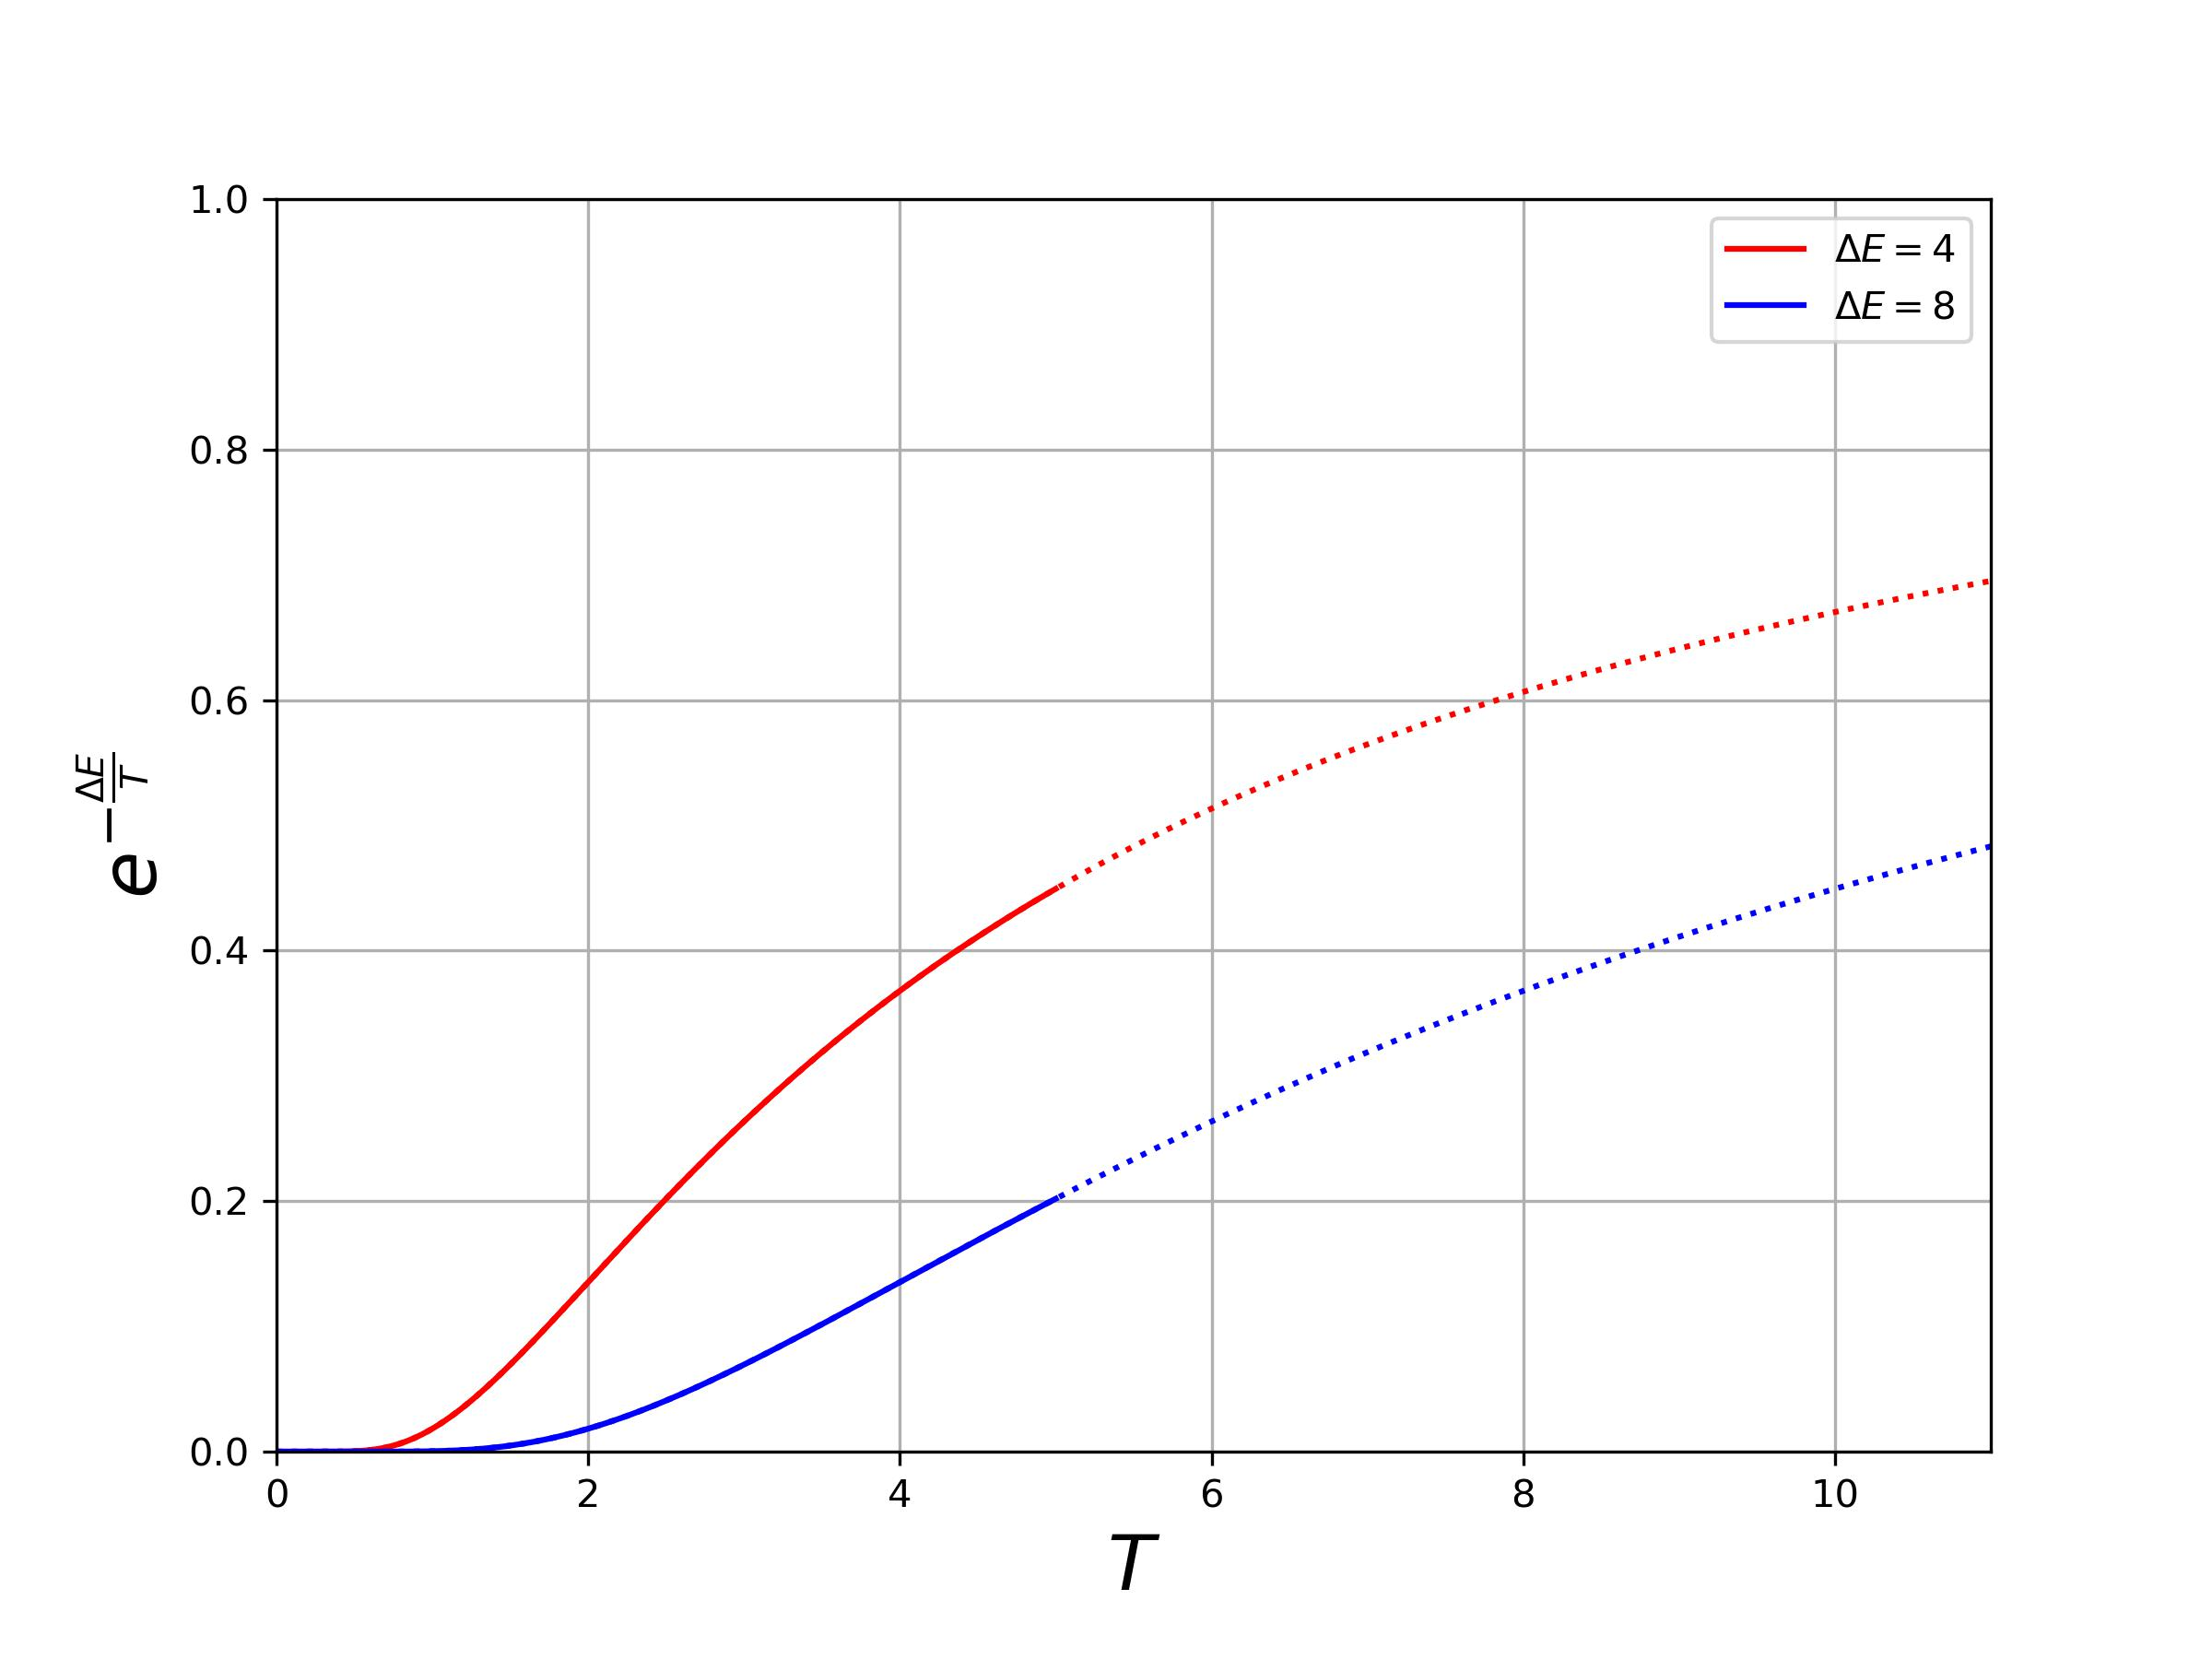
\includegraphics[width=0.5\linewidth]{proba.jpg}
	\caption{probabilité de transition en fonction de la température}
	\label{fig:H}
\end{figure}

On peut donc alors lancer la simulation, pour une température fixé on réalise un certains nombre de tentative de changement de spin. Le système va alors se relaxer jusqu'à un équilibre où la moyenne des spins qui composent l'image est stable tentative successive de changement de l'état d'un spin de l'image.

\begin{figure}[h]
	\centering
	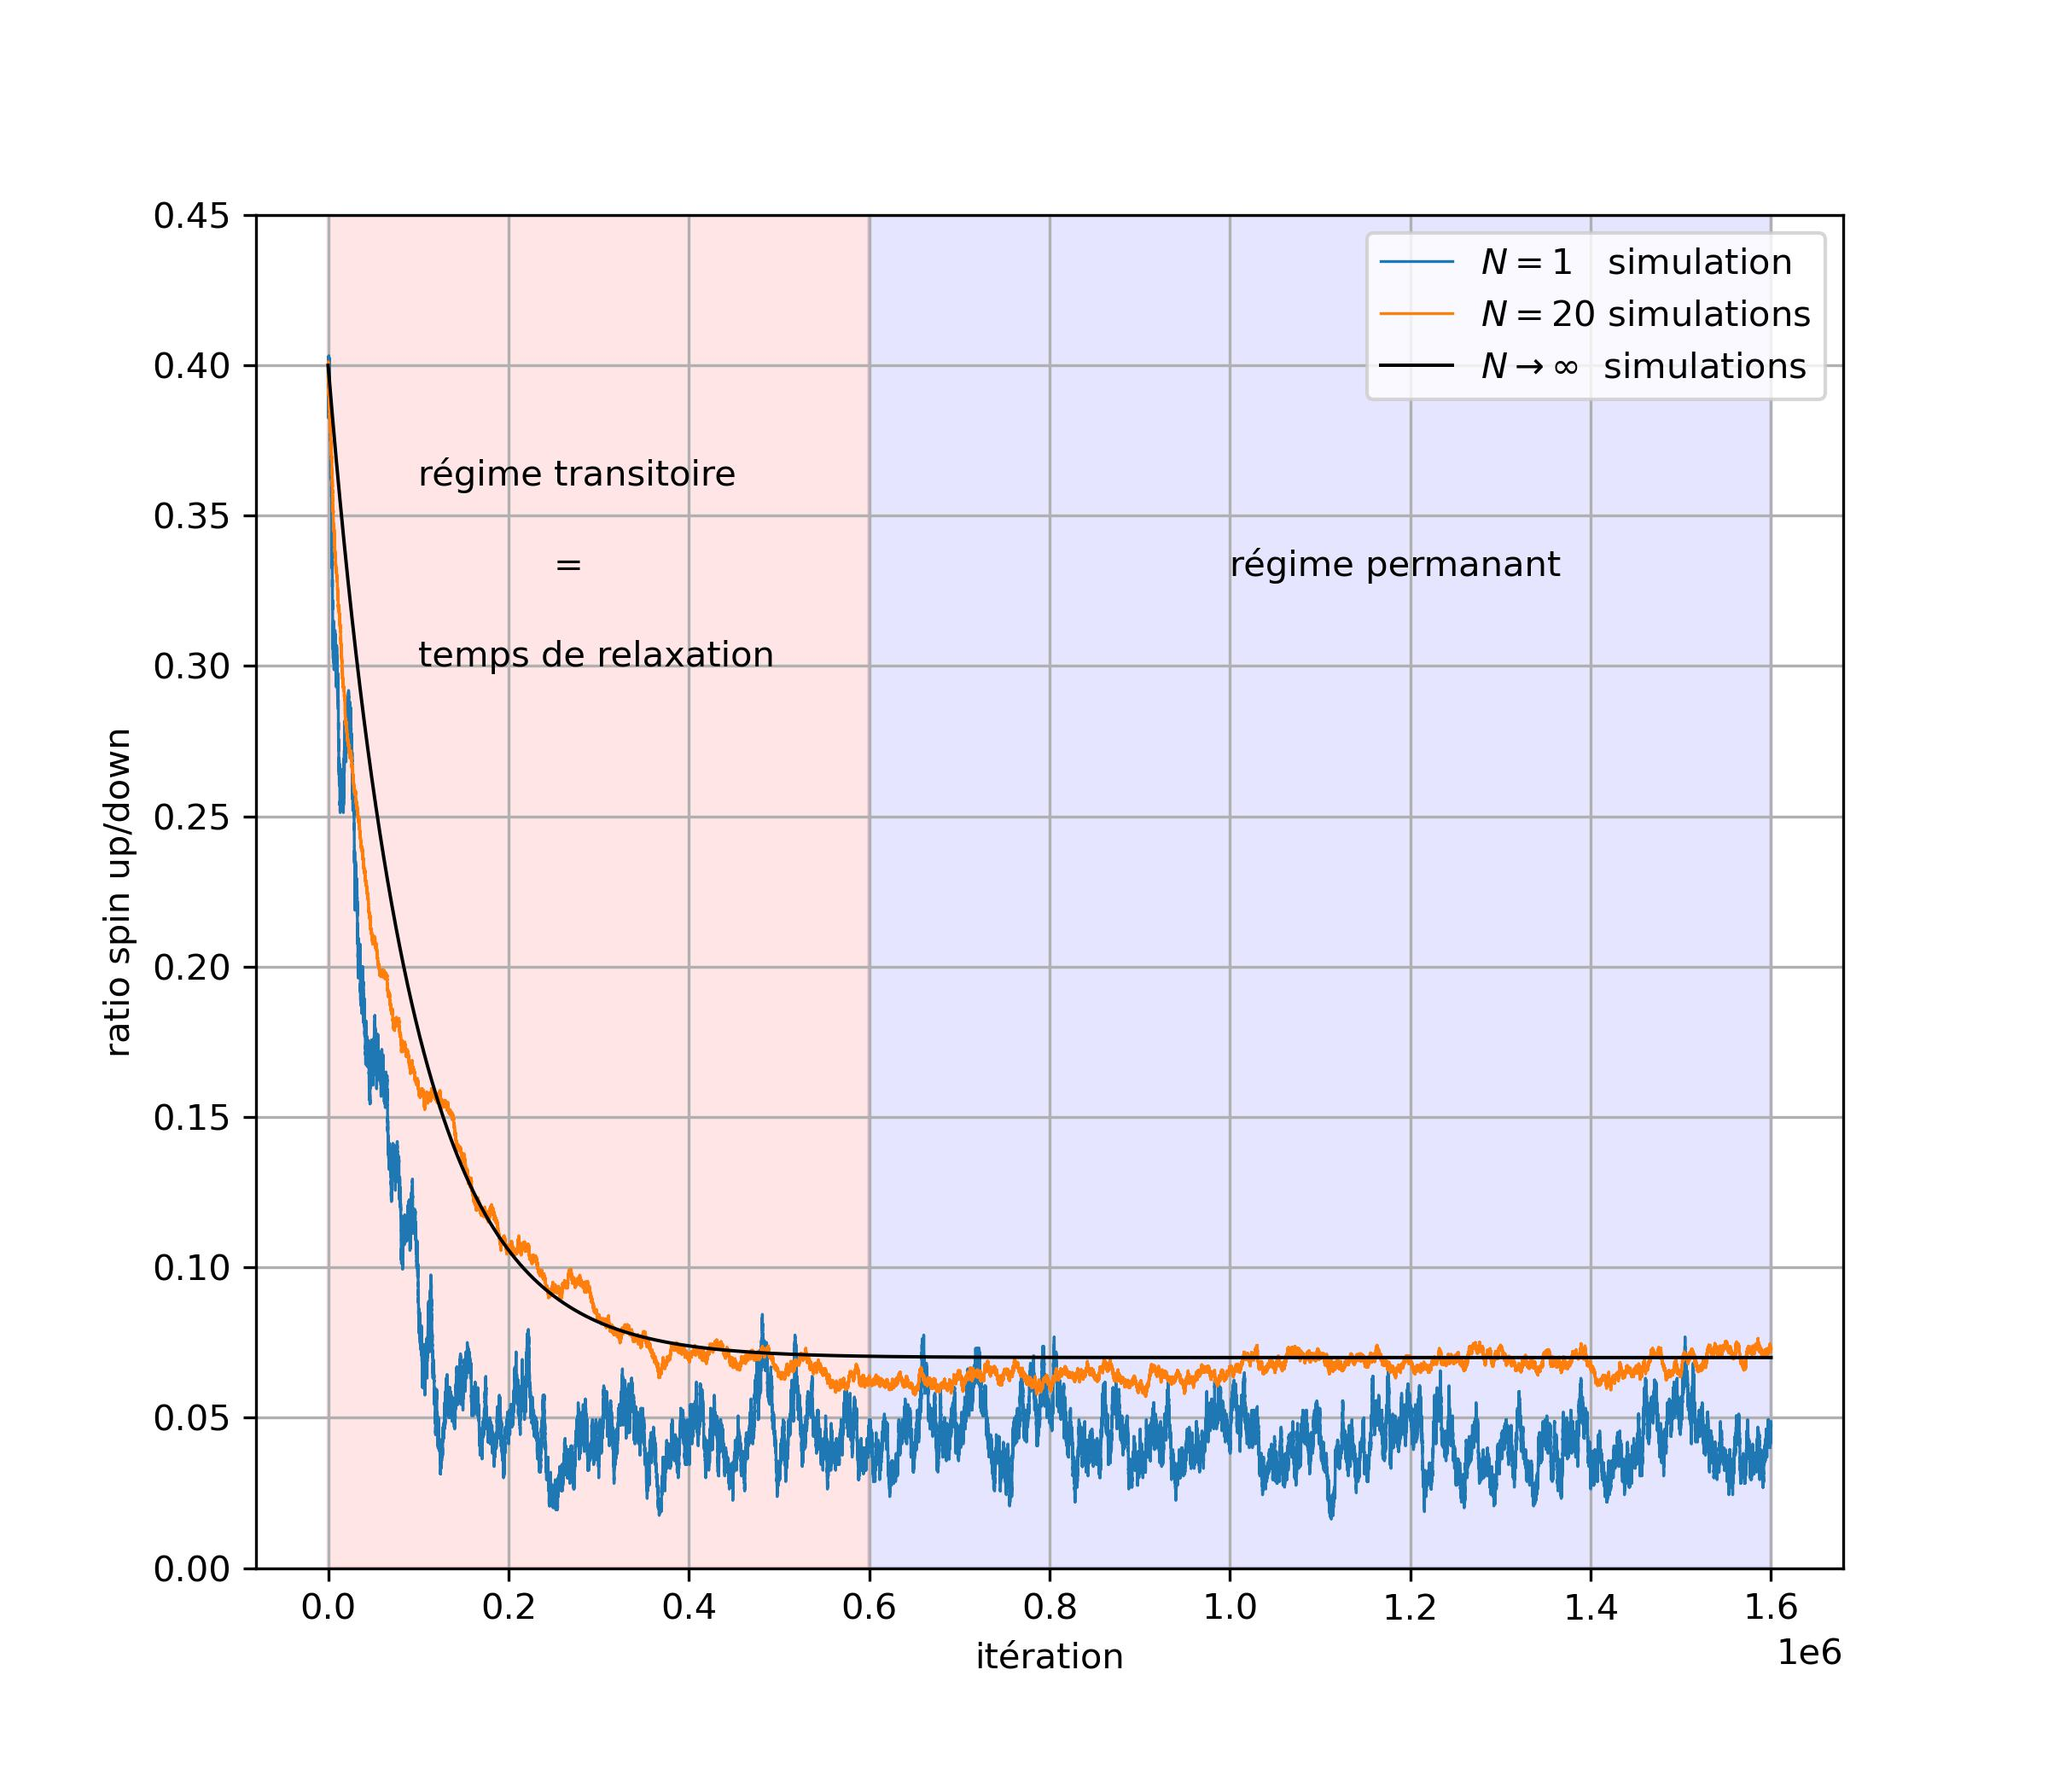
\includegraphics[width=0.5\linewidth]{simulation_ising.jpg}
	\caption{Évolution du ratio spin up spin down pour $T=2$ et $1,6$ million itération }
	\label{fig:H}
\end{figure}


\section{Pré-traitement des données}
Maintenant que nous avons généré nos données, nous devons nous faire une idée de la forme de nos données afin de pouvoir les traiter de la meilleure façon possible.
Les données fournies au départ sont des vecteurs de taille $1600$ contenant des $1$ et des $0$. Ces vecterus représentent des configurations de spins se trouvant sur une grille 2D de taille $40 \times 40$. Le dataset original est composé de $10000$ configurations de spins pour $16$ températures différentes comprises entre $0.25$ et $4.00$ avec un pas de $0.25$.
Avec ces configurations, un label est associé à chaque configuration. Ce label est une valeur binaire qui nous indique la phase dans laquelle se trouve le système. 
De plus, nous avons généré \todo{Anatole : Compléter cette ligne ou supprimer si superflu}...
Comme on peut le voir sur la figure \ref{fig:rawdata}, nos données forment un ensemble bruité mais il apparaît une symétrie par rapport à l'axe horizontal. En effet, à basse température, les spins sont majoritairement alignés de la même façon mais de manière aléatoire en $+$ ou $-$.
Cette symétrie de nos données peut poser un problème à nos modèles qui auront dû apprendre à faire la différence entre deux configurations opposées mais équivalentes. Pour éviter ce problème, nous allons symétriser nos données en inversant les spins de toutes les configurations qui ont une moyenne de spin \todo{Vérifier la manière de symétriser} négative. 
Ainsi, on se retrouve avec des données symétriques par rapport à l'axe horizontal comme on peut le voir sur la figure \ref{fig:symdata}.

\begin{figure}[h]
	\begin{subfigure}{0.5\textwidth}
		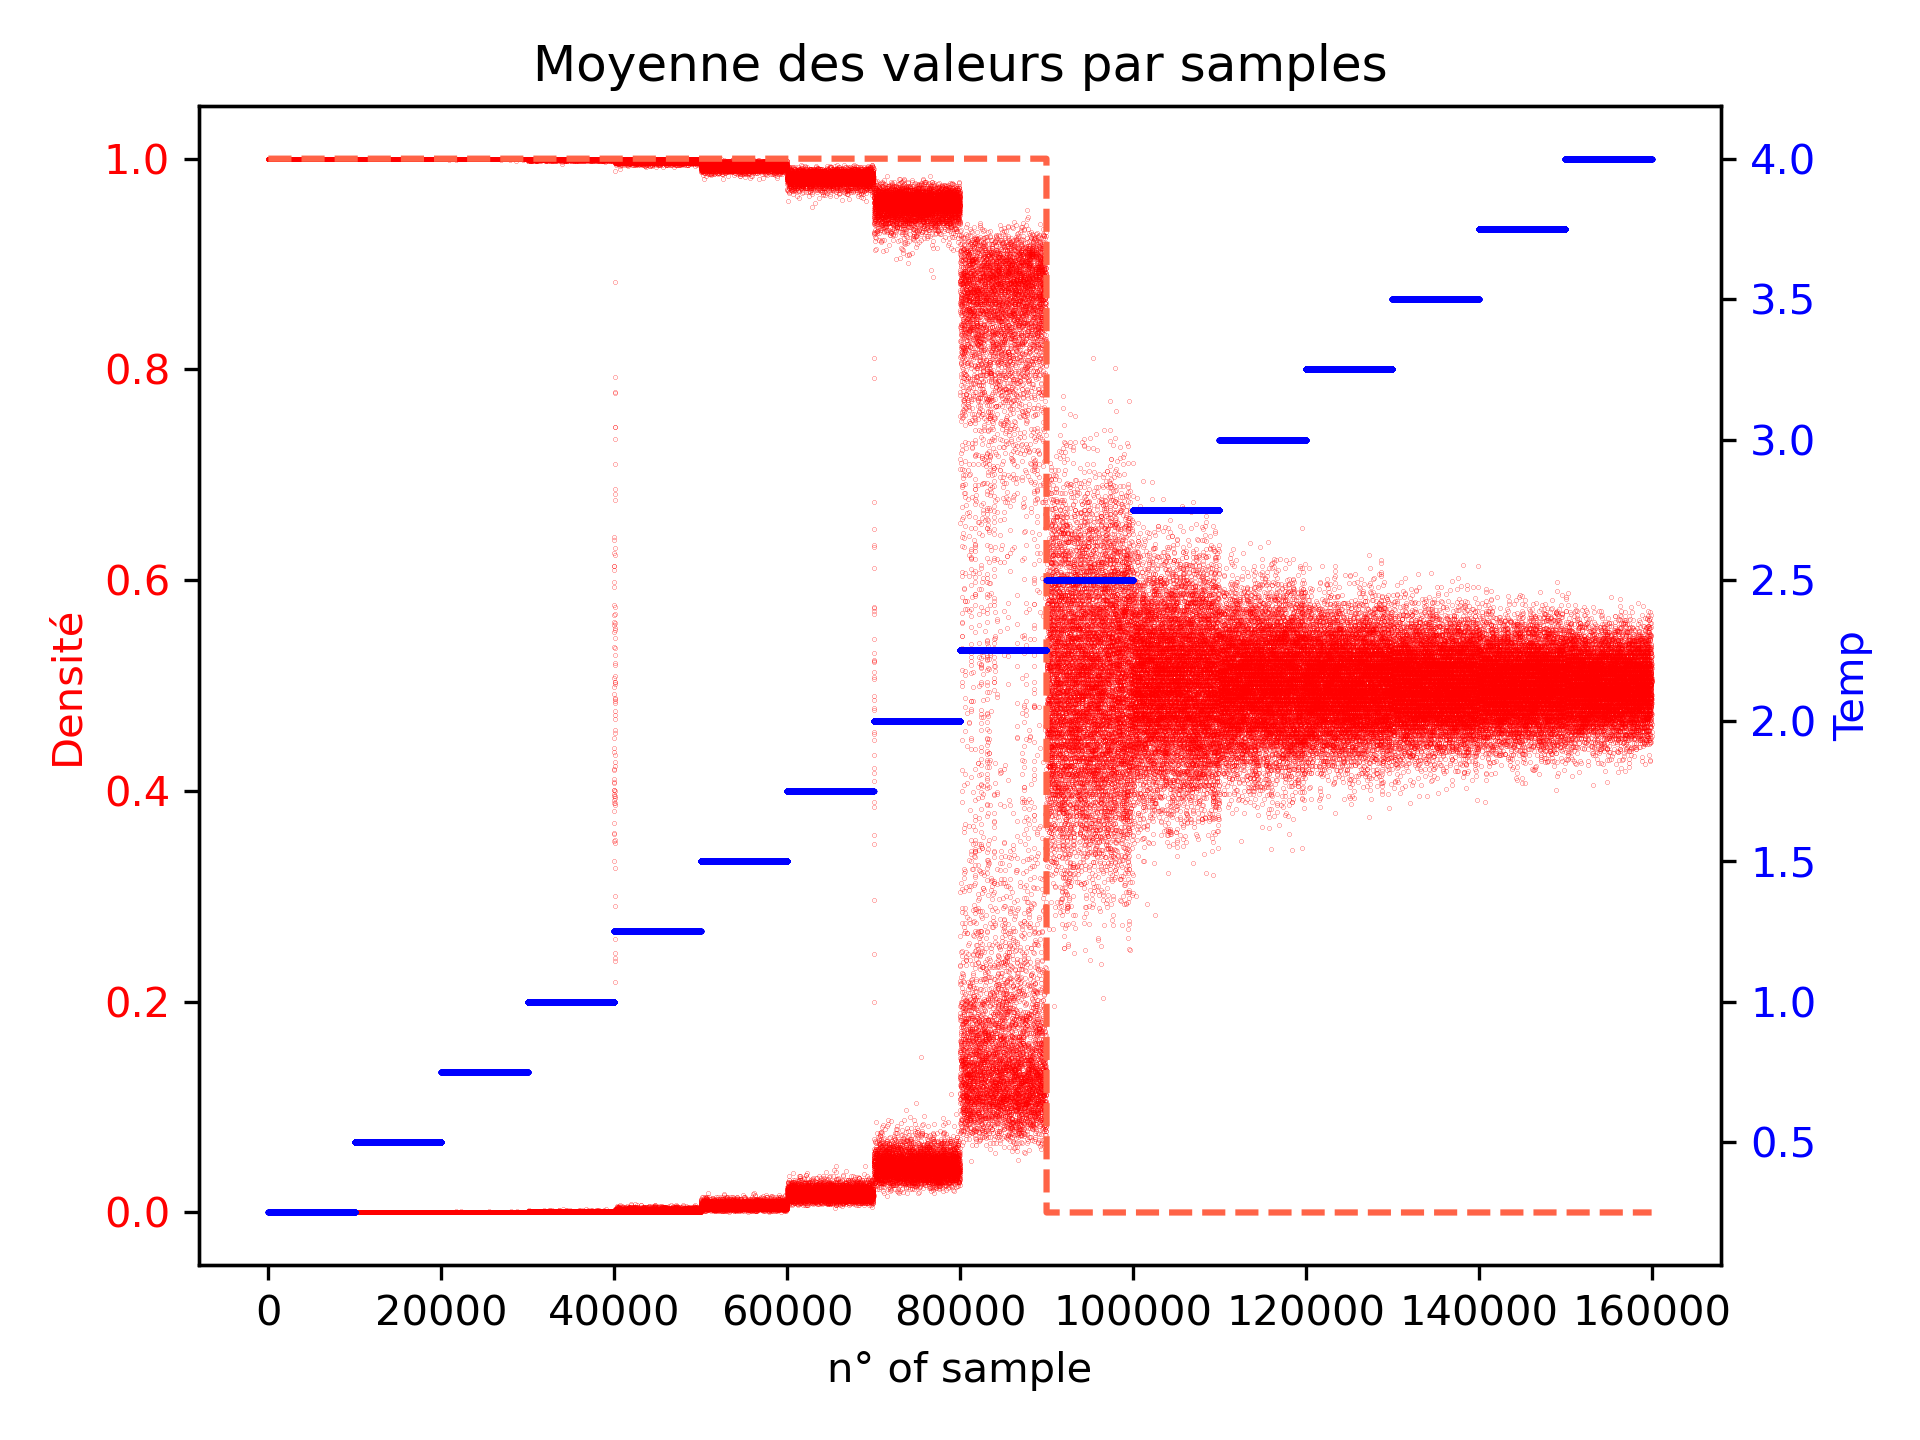
\includegraphics[width=0.95\linewidth]{./figures/raw_data.png}
		\caption{Données brutes}
		\label{fig:rawdata}
	\end{subfigure}
	\begin{subfigure}{0.5\textwidth}
		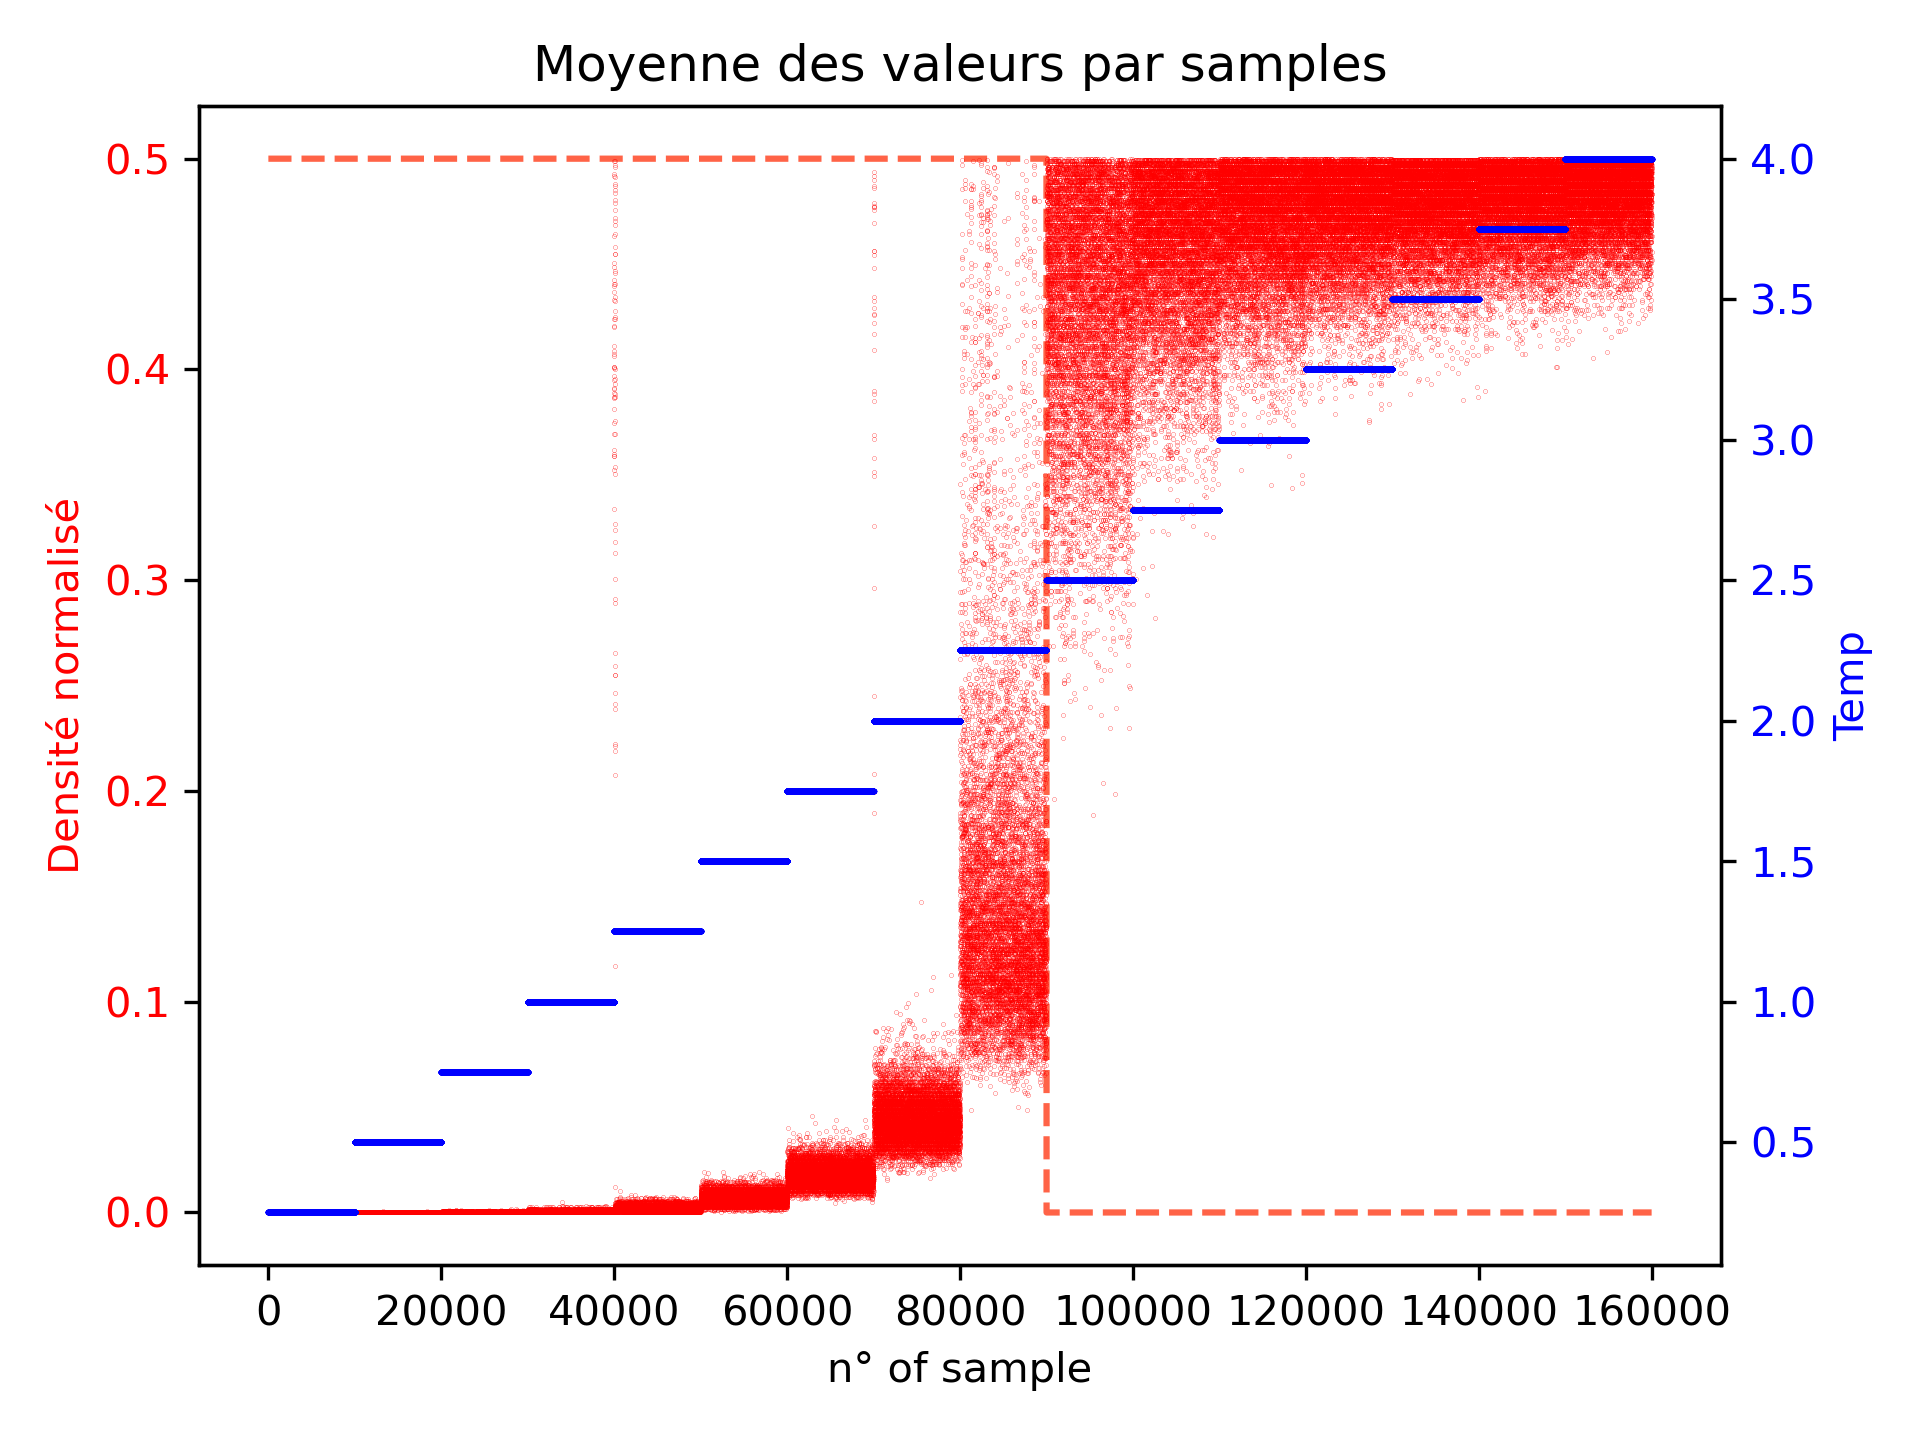
\includegraphics[width=0.95\linewidth]{./figures/sym_data.png}
		\caption{Données symétrisées}
		\label{fig:symdata}
	\end{subfigure}
	\caption{}
\end{figure}

Dans la partie suivante, nous allons entraîner certains modèles spécifiques sur la densité de spin symétrisée. Dans ce cas, nous allons aussi normaliser afin de rendre les modèles plus performants.
Pour cela, nous allons utiliser la méthode \textit{StandardScaler} de la librairie \textit{sklearn} qui permet de centrer et réduire les données. Cette méthode soustrait la moyenne et divise par l'écart-type. Ainsi, on se retrouve avec des données centrées en $0$ et de variance $1$.

Afin d'appliquer exactement la même transformation sur les données de test, nous allons créer un pipeline qui va appliquer la méthode de symétrisation puis la méthode de normalisation. Ainsi, on pourra appliquer le pipeline sur les données de test sans avoir à les modifier.
Finalement, certains modèles seront plus réceptifs à des données présentées sous forme de vecteur de taille $1600$, d'autre sous forme de matrice de taille $40 \times 40$. Pour éviter de devoir modifier les données à chaque fois, nous allons créer un pipeline qui va transformer les données en matrice si nécessaire et appliquer les autres méthodes de pré-traitement expliquées ci-dessus.

\section{Modèles classiques}

\subsection{Analyse par la magnétisation}
Notre première approche de ce problème est de considérer la magnétisation comme une fonction de la température. Cette approche nous permet de réduire grandement la complexité du problème. En effet, nous n'avons plus qu'une seule variable à considérer : l'état moyen des spins. Dans cette partie, nous allons donc essayer de prédire la température à partir de la magnétisation. Il suffit ensuite de comparer la valeur prédite à la valeur de la température critique pour déterminer la phase du système.

Avant tous, nous allons établir un modèle naif qui va nous servir de référence. Ce modèle va simplement renvoyer la valeur moyenne de la température du jeu de données. Ainsi, on pourra comparer les performances de nos modèles avec ce modèle naif. On obtient une erreur quadratique moyenne de $1.32$.

Du fait du bruit de nos données et du faible nombre de températures distinctes, nous devons porter une attention particulière au sur-apprentissage de nos modèles.
Prenant en compte le grand nombre de données, nous sommes partis sur un modèle de foret aléatoire. Ce modèle est très robuste et permet de limiter le sur-apprentissage. De plus, il est très rapide à entraîner et à tester. 
Au niveau des hyperparamètres, nous avons limité la profondeur des arbres à 5 et nous avons aussi composé la foret de $100$ arbres. De plus, la méthode de \textit{Bootsrap} est activée. Cette méthode permet de créer des sous-ensembles de données de la taille de l'ensemble de données originale. Ainsi, on peut entraîner plusieurs arbres sur des données différentes et les combiner pour obtenir un modèle plus robuste.
On peut donc limiter le sur-apprentissage tout en gardant un modèle performant. Les résultats obtenus sont présentés sur la figure \ref{fig:forest}.
La figure \ref{fig:forest} possède deux objets : La densité de points de la moyenne des spins symétrisée par température calculé en utilisant la méthode de \textit{kde} et la prédiction du modèle de foret aléatoire. 

Avec une MSE de $0.108$, on obtient un modèle qui est $12$ fois plus performant que le modèle naif. Cependant, on peut voir que le modèle a du mal à distinquer les hautes températures. En effet, les valeurs prédites par ce modèle sont toujours inférieures à $3.5$.
\todo[inline]{Completer avec explication de la partie d'Anatole}

\begin{figure}[h]
	\centering
	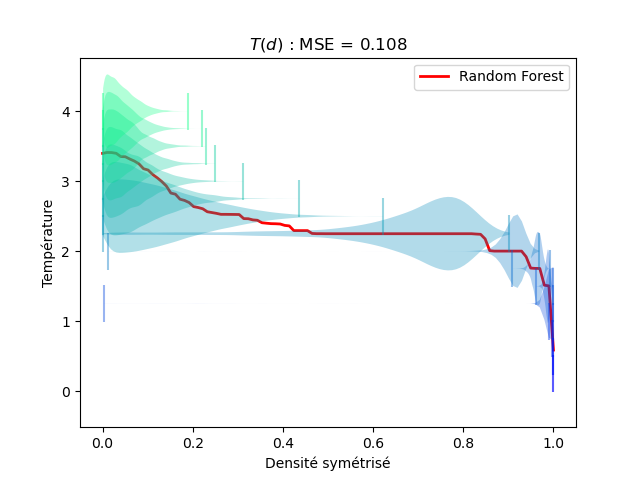
\includegraphics[width=0.75\linewidth]{./figures/forest.png}
	\caption{Résultats du modèle de foret aléatoire}
	\label{fig:forest}
\end{figure}

\subsection{Analyse par l'état individuel des spins}

\section{Réseaux de neurones}

\addcontentsline{toc}{section}{Conclusion}
\section*{Conclusion}

\end{document}